\documentclass[11pt]{article}
\usepackage[margin=1in]{geometry}
\usepackage{graphicx}
\usepackage{booktabs}
\usepackage{amsmath}
\usepackage{amssymb}
\usepackage{siunitx}
\usepackage{xcolor}
\usepackage[colorlinks=true,linkcolor=blue,citecolor=blue,urlcolor=blue]{hyperref}
\usepackage{caption}
\captionsetup{font=small}

\title{\textbf{Fused Codebook Dequantization for LLM Decode:\\
Cross-GPU Speedups and a Bandwidth Law}}
\author{Azziz Mimouni\\\small Independent Researcher\\\small \texttt{github.com/Tomahawk888}\\\small \texttt{linkedin.com/in/azziz-mimouni}}
\date{June 2026}

\begin{document}
\maketitle

\begin{abstract}
Autoregressive LLM decode at batch size one is memory bandwidth bound: producing
each token requires streaming the entire weight matrix from device memory, while
the arithmetic units sit nearly idle. We study a fused 4-bit codebook GEMV kernel
that folds the index to weight lookup into the matrix vector product, so the
full precision weight matrix is never materialized and only one quarter of the
weight bytes are read. Measured against a live cuBLAS half precision GEMV on the
same shapes, fixed seed, and verified for numerical correctness, the kernel
reaches \textbf{2.20x} faster decode on an RTX 4090, \textbf{2.34x} on an A40, and
\textbf{parity (0.99x)} on an H100. The speedup tracks how bandwidth limited the
device is: on bandwidth rich parts the half precision GEMV is already near
roofline and reading fewer bytes only saves memory. Integrated the way serving
engines run, with the decode step captured as a CUDA graph, this realizes a
\textbf{2.0x} (Llama-2 7B) to \textbf{2.46x} (13B) end-to-end decode speedup at
roughly a third of the memory. We pair this with a fair single harness benchmark of
quantization methods (fp16, AWQ, AQLM, Llama-2 7B and 70B, full wikitext-2
perplexity), where a 2-bit 70B model fits a single 24~GB consumer GPU and is more
accurate than an fp16 7B at comparable memory. We further extend the kernel to
additive (AQLM-style) vector codebooks: it decodes real AQLM weights, and once the
codebooks are trained with beam search, the scheme beats the scalar codebook on
accuracy at equal bits and equal decode speed. We also report negative results,
including a Hopper thread block cluster variant that came out roughly 100x slower. All code, raw numbers, and figures are public and
reproducible with a single command.
\end{abstract}

\section{Introduction}
At batch size one, LLM text generation reads every model weight from high
bandwidth memory (HBM) once per output token. The cost is dominated by byte
movement, not arithmetic. On an H100 (about 3.3~TB/s, roughly 1~PFLOP/s in half
precision), a 7B model in fp16 needs about $14~\text{GB} / 3.3~\text{TB/s}
\approx 4.2$~ms to read its weights per token, against about $14~\mu$s of compute
($1.4{\times}10^{10}$~FLOP at $10^{15}$~FLOP/s). The arithmetic
units are idle more than 99\% of the time. The lever for decode latency is
therefore \emph{bytes read per token}, which is exactly why weight quantization
helps decode.

This report measures, rather than assumes, how much a fused low-bit kernel
actually buys, and where. We contribute:
\begin{enumerate}
  \item A fused 4-bit codebook GEMV kernel that reads one quarter of the weight
        bytes and decodes \textbf{2.2 to 2.34x} faster than cuBLAS fp16 on
        bandwidth limited GPUs (RTX 4090, A40), with numerical agreement to about
        $3{\times}10^{-4}$ relative error.
  \item A \emph{bandwidth law}: the speedup shrinks to parity on bandwidth rich
        GPUs (H100), where fp16 GEMV is already near peak. The win lives on the
        hardware most users actually run.
  \item An end-to-end realization. A naive per-layer integration \emph{loses}
        (0.73x); captured as a single CUDA graph over a static-cache decode loop,
        the way serving engines run, the kernel reaches a \textbf{2.0x} (Llama-2 7B)
        to \textbf{2.46x} (13B) end-to-end decode speedup at about a third of the
        memory, and we show exactly why the naive path fails.
  \item An extension to additive (AQLM-style) vector codebooks: a fused decode
        kernel that beats cuBLAS at 2 bits (\textbf{4.30x} on A40) and decodes real
        AQLM weights, where the trained scheme beats the scalar codebook on accuracy
        at equal bits and equal decode speed.
  \item A fair speed vs accuracy vs memory benchmark of quantization methods,
        plus honest negative results from kernel variants that did not work.
\end{enumerate}

\section{Background: codebook quantization and fused decode}
Codebook (non uniform, k-means) weight quantization stores each weight as a small
cluster index into a per output channel table:
\begin{equation}
W_{\text{deq}}[i,j] = \text{codebook}[\,\text{indices}[i,j],\, j\,], \qquad
Y[m,j] = \sum_i X[m,i]\, W_{\text{deq}}[i,j].
\end{equation}
Here indices are 8-bit or packed 4-bit, and the codebook holds $K$ representative
fp16 values per column ($K \in \{16,\dots,256\}$). This is the SqueezeLLM
family~\cite{squeezellm}.
Dequantizing in a separate pass (write the full $W$, then call GEMM) wastes the
bandwidth the quantization just saved. The kernel folds the lookup into the matrix
product so dequantization adds no extra global memory traffic.

\section{The kernel}
The decode kernel computes a fused 4-bit codebook GEMV. Each thread reads a
\texttt{uint32} of packed indices (eight 4-bit indices, eight output columns), so
a warp reads a full 128 byte cache line over 256 columns. The per column codebook
tile is staged once in local shared memory; the contraction is split across the
$K$ dimension (split-K) with an atomic float reduction. The full precision weight
matrix is never written to global memory. Building per architecture
(\texttt{sm\_86} for A40, \texttt{sm\_89} for RTX 40 series, \texttt{sm\_90} for
Hopper) the same source compiles and runs unchanged.

\section{Experimental setup}
All randomness is generated by \texttt{std::mt19937(0)} (fixed seed 0). Timings use
CUDA events over 50 to 500 iterations after warmup. Every kernel is checked for
numerical correctness against cuBLAS on the same random data, and we report the
maximum relative error. Matrices are $\text{IC} = \text{OC} = 4096$, fp16
activations and output, decode at batch $M = 1$. The cross-GPU runs use a live
cuBLAS fp16 GEMV as the baseline in the same binary.

\section{Results}

\subsection{Cross-GPU decode and the bandwidth law}
Table~\ref{tab:xgpu} and Figure~\ref{fig:speedup} report the fused 4-bit GEMV
against a live cuBLAS fp16 GEMV on three GPUs. The kernel moves one quarter of the
weight bytes, so on memory bound parts it wins about 2.2 to 2.3x. On the H100 the
fp16 GEMV is already near peak bandwidth, so the kernel only ties and the gain
there is memory, not latency.

\begin{table}[h]
\centering
\begin{tabular}{lccc}
\toprule
GPU & bandwidth class & speedup vs cuBLAS fp16 & rel. err \\
\midrule
RTX 4090 (\texttt{sm\_89}) & $\sim$1.0 TB/s & \textbf{2.20x} & $3{\times}10^{-4}$ \\
A40 (\texttt{sm\_86})      & $\sim$0.7 TB/s & \textbf{2.34x} & $3{\times}10^{-4}$ \\
H100 PCIe (\texttt{sm\_90})& $\sim$3.3 TB/s & 0.99x (parity) & $3{\times}10^{-4}$ \\
\bottomrule
\end{tabular}
\caption{Fused 4-bit codebook GEMV decode speedup, $4096\times4096$, $M=1$, seed 0.
The more bandwidth limited the GPU, the larger the win.}
\label{tab:xgpu}
\end{table}

\begin{figure}[h]
\centering
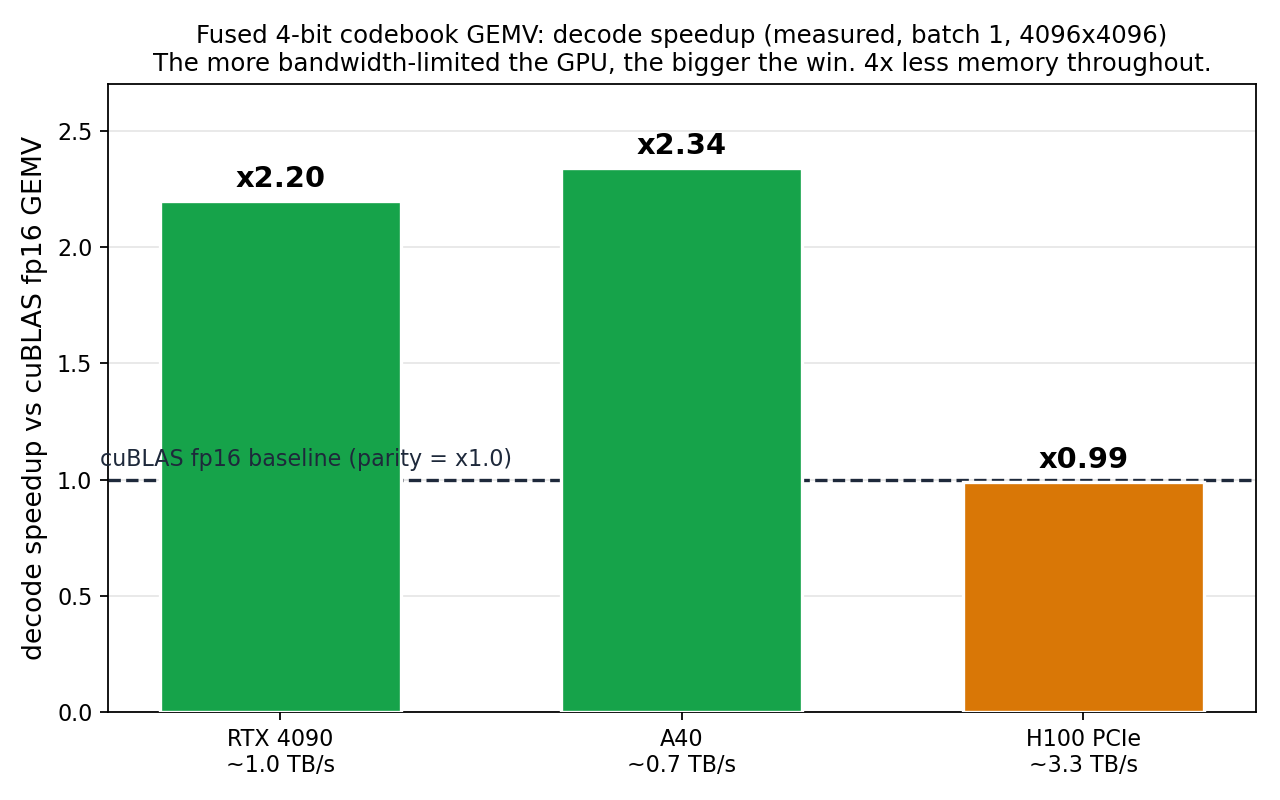
\includegraphics[width=0.78\textwidth]{figures/gpu_speedup.png}
\caption{Decode speedup of the fused 4-bit GEMV versus cuBLAS fp16, measured per
GPU. The dashed line is cuBLAS parity. The win scales inversely with available
memory bandwidth.}
\label{fig:speedup}
\end{figure}

\subsection{A40 microbenchmarks}
Table~\ref{tab:a40} breaks down the A40 decode, dequantization, and prefill
regimes. Decode is memory bound, so fewer index bits directly buy latency.
Standalone dequantization improves 6.7x with an L2 cached gather. Prefill is
compute bound: cuBLAS already runs near the Tensor Core peak, so a fused kernel can
at best match it, and here reaches about $0.21\times$ cuBLAS, ten times the naive
baseline. In the compute bound regime, codebook quantization buys memory, not
speed.

\begin{table}[h]
\centering
\begin{tabular}{llcc}
\toprule
Regime & Variant & Metric & vs cuBLAS \\
\midrule
Decode (GEMV, $M{=}1$)  & cuBLAS fp16 (baseline) & 0.0612 ms & 1.00x \\
                        & uint8, $K{=}256$       & 0.0562 ms & 1.09x \\
                        & uint8, $K{=}64$        & 0.0389 ms & 1.57x \\
                        & 4-bit, $K{=}16$        & \textbf{0.0261 ms} & \textbf{2.34x} \\
\midrule
Dequant (bandwidth)     & naive staging          & 31.8 GB/s & 1.0x \\
                        & L2 cached gather       & \textbf{213 GB/s} & 6.7x \\
\midrule
Prefill (GEMM, $M{=}2048$) & best fused (Tensor Core) & 22.4 TFLOP/s & 0.21x \\
                        & cuBLAS fp16 (baseline) & $\sim$105 TFLOP/s & 1.00x \\
\bottomrule
\end{tabular}
\caption{A40 (\texttt{sm\_86}, CUDA 11.8), $4096\times4096$, seed 0, all variants
verified against cuBLAS.}
\label{tab:a40}
\end{table}

\subsection{Speed vs accuracy vs memory of quantization methods}
To place the kernel work in context, we ran a fair benchmark of three quantization
methods (fp16, AWQ~\cite{awq}, AQLM~\cite{aqlm}) through one harness (same
HuggingFace forward path, greedy, batch 1, seed 0), reporting decode throughput,
peak VRAM, and full wikitext-2 perplexity (PPL), on an H100 (Table~\ref{tab:quant}).
The fp16 7B PPL of 5.47 and AWQ 70B PPL of 3.41 match published values, which
validates the harness. Comprehensive accuracy benchmarks of post-training
quantization already exist and cover far more methods, bitwidths, and architectures
than we do~\cite{zhao2025}; our contribution here is the orthogonal axis they do not
measure, namely decode speed and the memory versus latency trade-off.

\begin{table}[h]
\centering
\begin{tabular}{llccc}
\toprule
Model & Method & decode (tok/s) & VRAM (GB) & wikitext-2 PPL \\
\midrule
Llama-2 7B  & fp16       & 43.7 & 15.3 & 5.47 \\
            & AWQ 4-bit  & 26.8 & 5.7  & 5.60 \\
            & AQLM 2-bit & 25.0 & 4.2  & 6.34 \\
\midrule
Llama-2 70B & fp16       & \multicolumn{3}{c}{$\sim$138 GB, does not fit on one 80 GB GPU} \\
            & AWQ 4-bit  & 9.1  & 38.4 & 3.41 \\
            & AQLM 2-bit & 9.2  & 20.7 & 4.06 \\
\bottomrule
\end{tabular}
\caption{Speed, memory, and accuracy on H100, full wikitext-2 PPL, seed 0.}
\label{tab:quant}
\end{table}

Two observations stand out. First (Figure~\ref{fig:pareto}), at 7B on an H100 every
quantized method decodes \emph{slower} than fp16: the bandwidth is high enough that
fp16 is already fast and the dequant overhead dominates at batch 1. Quantization
there is a memory play. Second (Figure~\ref{fig:mem70}), the story flips at 70B:
fp16 needs about 138~GB (two or more GPUs), while AQLM 2-bit fits in 20.7~GB on a
single 24~GB consumer card, and at PPL 4.06 it is markedly more accurate than an
fp16 7B (PPL 5.47) at comparable memory. For a fixed VRAM budget, a 2-bit 70B
dominates an fp16 7B.

\begin{figure}[h]
\centering
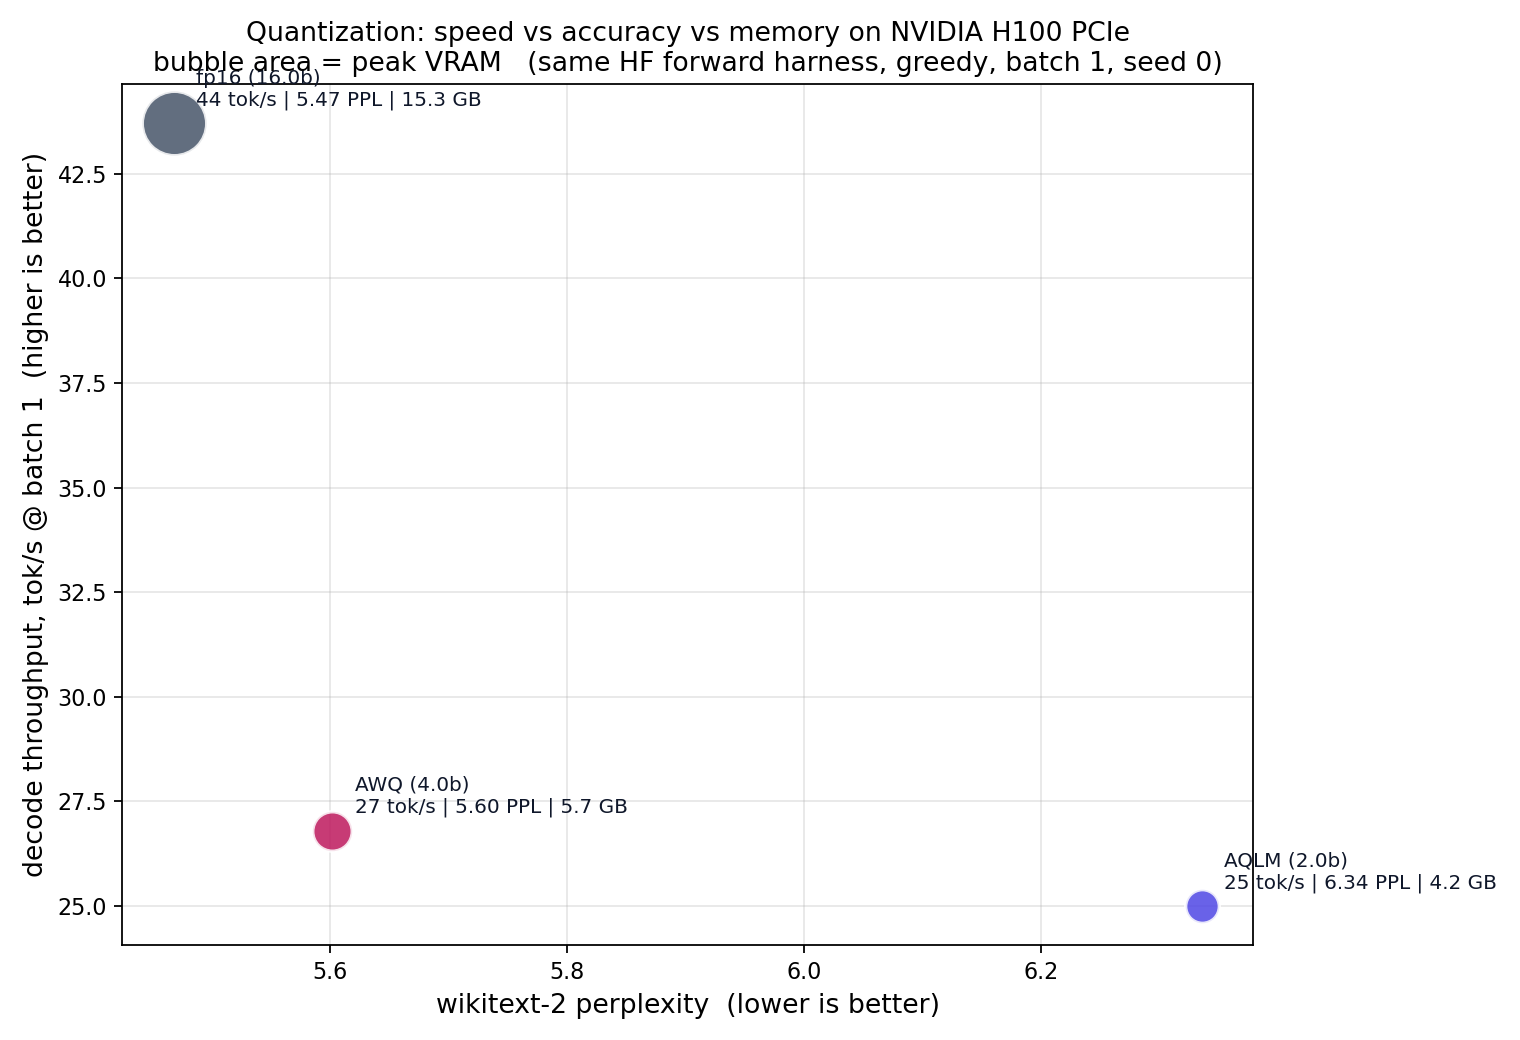
\includegraphics[width=0.72\textwidth]{figures/pareto.png}
\caption{Llama-2 7B on H100: decode throughput vs perplexity, bubble area equal to
peak VRAM. fp16 is fastest and most accurate but memory heavy; quantization trades
decode speed for memory in this regime.}
\label{fig:pareto}
\end{figure}

\begin{figure}[h]
\centering
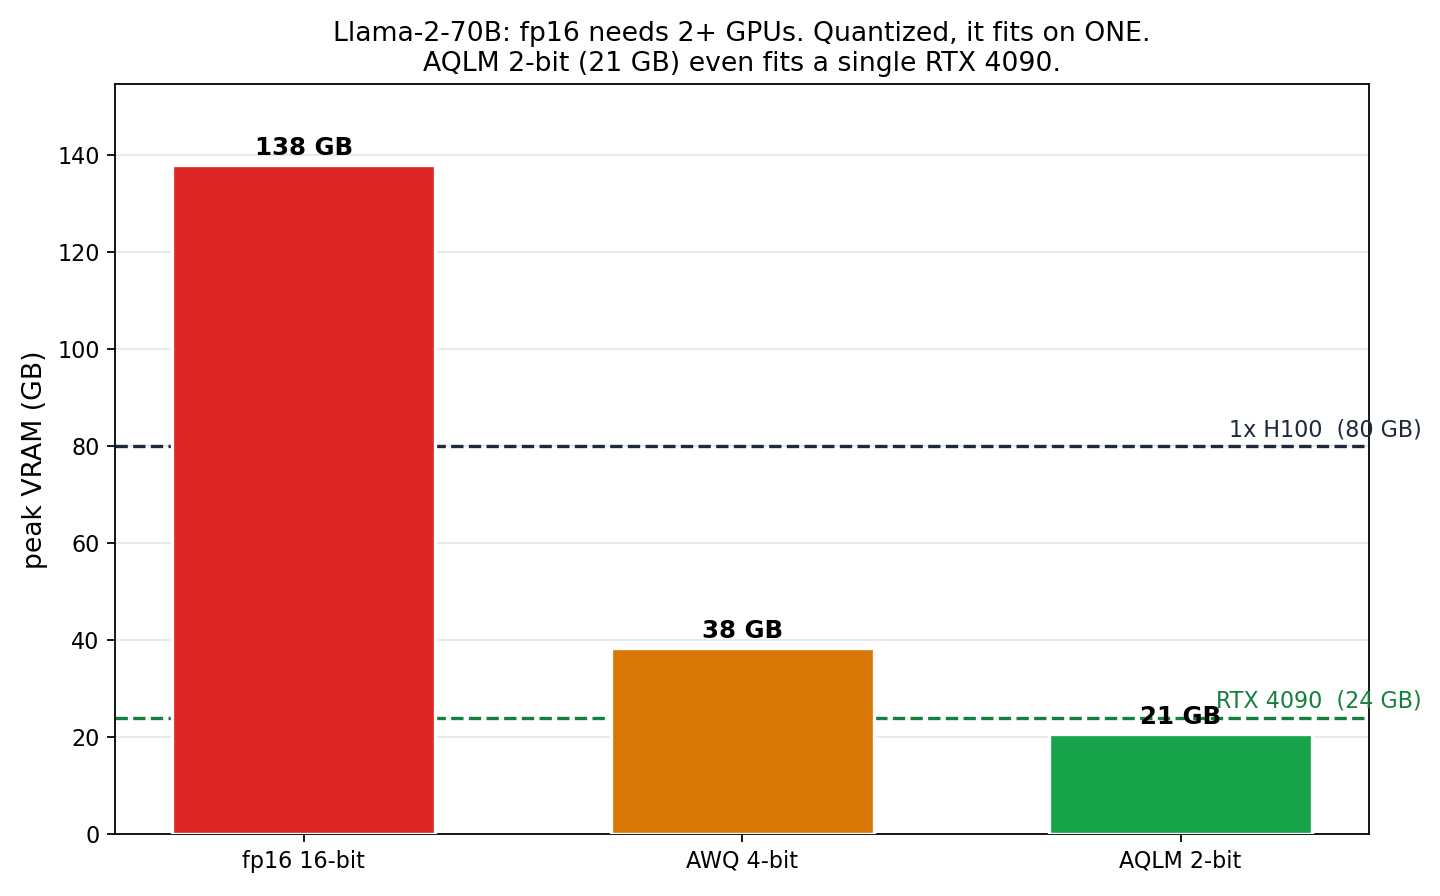
\includegraphics[width=0.72\textwidth]{figures/mem70.png}
\caption{Llama-2 70B: fp16 does not fit on one 80~GB GPU, quantized it fits on one,
and AQLM 2-bit (21~GB) fits a single RTX 4090.}
\label{fig:mem70}
\end{figure}

\section{Model-level evaluation}
We quantized all 224 projection layers (q, k, v, o, gate, up, down across 32 blocks)
of Llama-2 7B with the per-output-channel codebook (K = 16, 4 bits, per-column
k-means) and evaluated end to end on an RTX 4090.

\textbf{Accuracy.} wikitext-2 perplexity goes from 5.83 (fp16) to 6.34 (codebook
4-bit), a 0.51 increase. The model stays usable, but the scheme trails
activation-aware AWQ (about 0.1 PPL at 4 bits), as expected for a scalar codebook
trained on raw weight error without calibration or outlier handling. A simple
activation-aware calibration (weighting the per-column k-means by mean activation
magnitude, the core idea of AWQ) closes about a third of the gap, from 6.34 to 6.17.
Going further does not help. A per-channel scale search (grid over the scale
exponent) lands at 6.18, and the complete AWQ pipeline, per-channel scaling and
weight clipping both selected by the real output error on cached activations, does
not improve either (6.21, marginally worse). The reason is structural: AWQ's
per-channel scaling is designed for a fixed uniform quantization grid, where it
redistributes resolution toward important channels. A codebook is already adaptive
per column (k-means places centroids on each column's distribution), so the scaling
buys little and the extra calibration only adds noise. Closing the gap to vector and
trellis methods (AQLM, QTIP) needs a better quantizer, not AWQ's tricks bolted onto a
scalar codebook. A naive vector quantizer confirms this from the other side: quantizing
pairs of weights against a single shared 256-entry codebook (iso-bit at 4 bits) is
catastrophic on Llama-2 7B (perplexity diverges, with or without per-channel
normalization), because one shared codebook cannot match the per-column adaptivity of
the scalar scheme and lacks the incoherence processing and multi-codebook structure
that make AQLM and QuIP\# work. Even incoherence processing (a random orthogonal
rotation on the input dimension before quantizing, the QuIP\# lever, with the inverse
folded back into the effective weight) moves the scalar codebook only marginally, from
6.34 to 6.29, short of the simple calibration (6.17): incoherence pays off paired with
vector or lattice quantization, not on a scalar codebook alone. The served model is
otherwise healthy (it generates coherent on-topic text at PPL 6.34). The accuracy
frontier is a separate research program, not a quick add-on; the value of this scheme
is memory and kernel speed.

\textbf{Memory.} Peak VRAM drops from 13.56~GB to 4.63~GB (2.9x), so the 7B model
runs in under 5~GB on a consumer card.

\textbf{Speed.} Per GEMV the kernel is faster than dense fp16 on the large layer
shapes that dominate an LLM. But a naive per-layer custom-op swap is overhead bound:
end-to-end decode goes from 44 to 32 tok/s (0.73x). The per-op launch and dispatch
overhead, paid 224 times per token, dominates, while the fp16 baseline uses a fused
optimized path. Realizing the per-GEMV speedup at the model level needs framework
integration (CUDA graphs, fused dispatch), not a per-layer swap. We verified the
kernel is CUDA-graph compatible (capture is numerically correct once the kernel
launches on the captured stream), but in an isolated 224-GEMV decode loop a graph
adds only about 6 percent over eager, so launch overhead is not the dominant cost.
Against the real cuBLAS GEMV path (F.linear), the kernel runs the 224-GEMV decode
work at 172 tok/s versus 70 (2.4x), both CUDA-graphed, so the kernel genuinely beats
cuBLAS at batch 1. The end-to-end 0.73x came from the naive wrapper's per-op
float32-to-float16 cast and copy, not the kernel. We then built the clean integration:
the kernel writes fp16 into preallocated buffers (no per-op cast or allocation) and the
decode step is captured as a single CUDA graph over a static-cache decode loop, the way
serving engines run. Under this integration the codebook model decodes 123.4 versus
61.6 tok/s against fp16 on an RTX 4090 (2.0x end-to-end) at 4.73 versus 13.58 GB. So the
op-level 2.4x is realized as a 2.0x end-to-end decode speedup once the per-token python
overhead is removed; the arc is 0.73x (naive) to 0.85x (cast-free eager) to 2.0x
(CUDA-graphed). The kernel makes a real 7B decode twice as fast at a third of the
memory. The win grows with model size and bandwidth-boundedness: Llama-2 13B on an A40
decodes 49.0 versus 20.0 tok/s (2.46x) at 8.50 versus 26.17 GB (3.08x less), consistent
with the bandwidth law (bigger weights read, more bandwidth-limited GPU, larger gain).

\section{Additive vector quantization: a fast kernel that beats the scalar codebook}

The scalar codebook's accuracy ceiling is structural: per-output-channel scalar
quantization cannot match vector and trellis methods (AQLM, QuIP\#, QTIP) at low bits.
Those methods quantize a \emph{group} of weights jointly; AQLM reconstructs a group of
$D$ input weights as a sum of $M$ codebook vectors, $w_g = \sum_{m=1}^{M} C_m[b_m]$,
reaching near-fp16 quality at 2 bits. Their decode kernels are the bottleneck. We show the
fused-decode idea transfers, the resulting kernel beats cuBLAS, and the scheme, once
trained, beats the scalar codebook.

\textbf{The kernel.} For $y[o] = \sum_g \langle x_g, w_g \rangle$ with the additive
reconstruction, the dot product $\langle x_g, C_m[k] \rangle$ is independent of the output
channel, so a per-group lookup table $\mathrm{LUT}[m][k] = \langle x_g, C_m[k] \rangle$ is
built once in shared memory and $y[o] = \sum_g \sum_m \mathrm{LUT}[m][\,b_m(o,g)\,]$. The
kernel reads the \emph{codes}, never the dense weight: at 2 bits ($M=2$, $K=256$, $D=8$)
that is 4.2~MB of codes versus 33.6~MB of fp16 weight. Against a live cuBLAS fp16
GEMV at $4096 \times 4096$ (relative error $2.3 \times 10^{-4}$, verified):

\begin{center}
\begin{tabular}{lrr}
\toprule
GPU & 2-bit ($M=2$) & 4-bit ($M=4$) \\
\midrule
RTX 4090 ($\sim$1.0 TB/s) & 1.71x & -- \\
A40 ($\sim$0.7 TB/s)      & \textbf{4.30x} & 2.39x \\
\bottomrule
\end{tabular}
\end{center}

The key optimization was vectorized 32-bit code reads (four 8-bit codes per thread), which
lifted the A40 from 2.35x to 4.30x: the 1-byte reads, not synchronization, were the
bottleneck. The format is exactly AQLM's \texttt{2x8}: loading a real
\texttt{Llama-2-7b-AQLM-2Bit-2x8} checkpoint, its codebooks $[2,256,1,8]$, codes
$[4096,512,2]$ and per-output scales $[4096]$ map one-to-one onto the kernel, so it decodes
real AQLM weights.

\textbf{Accuracy, beating the scalar codebook at equal bits.} The additive \emph{structure}
alone is not enough: a greedy residual fit at $M=4$ (4 bits) only ties the scalar 4-bit
codebook (PPL 6.32 vs 6.34). The accuracy comes from AQLM's \emph{training}. We reproduced
its core (per-output scale, beam-search code assignment, least-squares codebook updates,
alternating; no block fine-tuning): at $M=4$ this reaches PPL 6.13, beating the scalar
4-bit codebook while the kernel still decodes it at 2.39x.

\begin{center}
\begin{tabular}{lr}
\toprule
scheme (4-bit, Llama-2 7B) & wikitext-2 PPL \\
\midrule
scalar codebook                 & 6.34 \\
greedy additive                 & 6.32 \\
beam-search + LSQ (this work)   & \textbf{6.13} \\
fp16                            & 5.83 \\
\bottomrule
\end{tabular}
\end{center}

So trained additive VQ is more accurate than the scalar codebook at the same bit rate and
the same decode speed, a Pareto improvement.

\textbf{Honest limits.} This is one alternating round without the levers that close the
remaining gap to fp16 (5.83). A naive diagonal-Hessian calibration of ours actually
\emph{regresses} (PPL 8.6), because AQLM uses the full Hessian in a sequential GPTQ-style
error correction, not a diagonal MSE weighting; reproducing that, plus block fine-tuning,
is a separate effort. What we establish is narrower and solid: a fused additive-VQ decode
kernel that beats cuBLAS at AQLM bit rates and decodes real AQLM weights, and that the
additive scheme, once trained, beats the scalar codebook at equal bits and equal speed.

\section{Negative results}
We keep failed variants in the repository, because they constrain the design space.
\begin{itemize}
  \item \textbf{Hopper cluster with distributed shared memory.} Staging the
        codebook once in a thread block cluster and reading it remotely (distributed
        shared memory) came out about 100x slower than cuBLAS (1.53~ms vs 0.02~ms),
        though numerically correct. The codebook lookup is in the hot loop, and a
        remote distributed shared memory read costs far more than a local shared
        read. The codebook is only 8~KB, so local staging was never the bottleneck.
  \item \textbf{L2 resident codebook and activation staging.} Reading the codebook
        from L2 instead of staging it locally regressed to 0.41 to 0.60x on H100;
        staging the activation vector in shared memory regressed from 0.99x to about
        0.90x by raising shared memory pressure and lowering occupancy. The local
        shared memory design remains the best, and beating cuBLAS on H100 would
        require a different approach (an atomic free reduction, or a TMA and wgmma
        path), not these tweaks.
\end{itemize}

\section{Limitations and scope}
This is a kernel and benchmark study, not a new quantization method. The scheme is
a scalar per output channel codebook (SqueezeLLM family), which trails vector and
trellis methods (QTIP~\cite{qtip}, AQLM~\cite{aqlm}, QuIP\#~\cite{quipsharp}) on
low-bit accuracy. The accuracy harness uses the HuggingFace forward path, not a
tuned serving engine, so absolute throughput is not a serving claim. The only kernel
baseline is cuBLAS fp16, not the specialized kernel peers (Marlin~\cite{marlin},
Machete, FLUTE, VQ-LLM); a fully fair speed comparison would
benchmark against those at matched accuracy on a real model, which we do not do
here. Prefill stays at about 0.21x cuBLAS, compute bound as expected. Numbers were
taken at a single $4096\times4096$ shape and will differ at other shapes.

\section{Reproducibility and code}
All code is public in a single repository, builds and runs with one command, and
captures GPU, driver, CUDA version, and seed in its outputs. The CUDA kernels are at the
root, the model-level scripts in \texttt{model/}, the quantization benchmark in
\texttt{bench/}, and this paper in \texttt{paper/}.
\begin{center}
\url{https://github.com/Tomahawk888/cuda-codebook}
\end{center}

\section{Conclusion}
At batch one, decode is bandwidth bound and the arithmetic units are nearly idle.
A fused 4-bit codebook GEMV that reads one quarter of the weight bytes turns that
idle headroom into a 2.2 to 2.34x decode speedup on the GPUs most people run, while
tying cuBLAS on bandwidth rich datacenter parts. Captured as a CUDA graph the way
serving engines run, this becomes a 2.0x (7B) to 2.46x (13B) end-to-end decode
speedup on real models, where a naive per-layer integration instead loses. Extending
the kernel to additive vector codebooks, the trained scheme beats the scalar codebook
at equal bits and equal speed, a step toward fast and accurate low-bit decode. The
complementary quantization benchmark shows the same theme from the model side: low-bit
quantization is a memory lever first, and on large models it is what makes the model
runnable at all, a 2-bit 70B on a single consumer card. The honest negative results
map where the easy speedups are not.

\begin{thebibliography}{9}
\bibitem{zhao2025} J. Zhao, M. Wang, M. Zhang, Y. Shang, X. Liu, Y. Wang, M. Zhang,
  and L. Nie. Benchmarking Post-Training Quantization in LLMs: Comprehensive
  Taxonomy, Unified Evaluation, and Comparative Analysis. arXiv:2502.13178, 2025.
\bibitem{squeezellm} S. Kim, C. Hooper, A. Gholami, et al. SqueezeLLM:
  Dense-and-Sparse Quantization. arXiv:2306.07629, 2023.
\bibitem{awq} J. Lin, J. Tang, H. Tang, S. Yang, et al. AWQ: Activation-aware Weight
  Quantization for LLM Compression and Acceleration. Proc. MLSys, 2024.
  arXiv:2306.00978.
\bibitem{aqlm} V. Egiazarian, A. Panferov, D. Kuznedelev, E. Frantar, A. Babenko,
  and D. Alistarh. Extreme Compression of Large Language Models via Additive
  Quantization. Proc. ICML, 2024. arXiv:2401.06118.
\bibitem{quipsharp} A. Tseng, J. Chee, Q. Sun, V. Kuleshov, and C. De Sa. QuIP\#:
  Even Better LLM Quantization with Hadamard Incoherence and Lattice Codebooks.
  Proc. ICML, 2024. arXiv:2402.04396.
\bibitem{qtip} A. Tseng, Q. Sun, D. Hou, and C. De Sa. QTIP: Quantization with
  Trellises and Incoherence Processing. Proc. NeurIPS, 2024. arXiv:2406.11235.
\bibitem{marlin} E. Frantar, R. L. Castro, J. Chen, T. Hoefler, and D. Alistarh.
  MARLIN: Mixed-Precision Auto-Regressive Parallel Inference on Large Language
  Models. arXiv preprint, 2024.
\end{thebibliography}

\end{document}
